El programa desarrollado para el análisis de películas radiocrómicas proporciona varias funcionalidades para el usuario. En la figura \ref{fig:ventanaPrincipal} se muestra la venta principal del programa.\\
\begin{figure}[H]
	\centering
	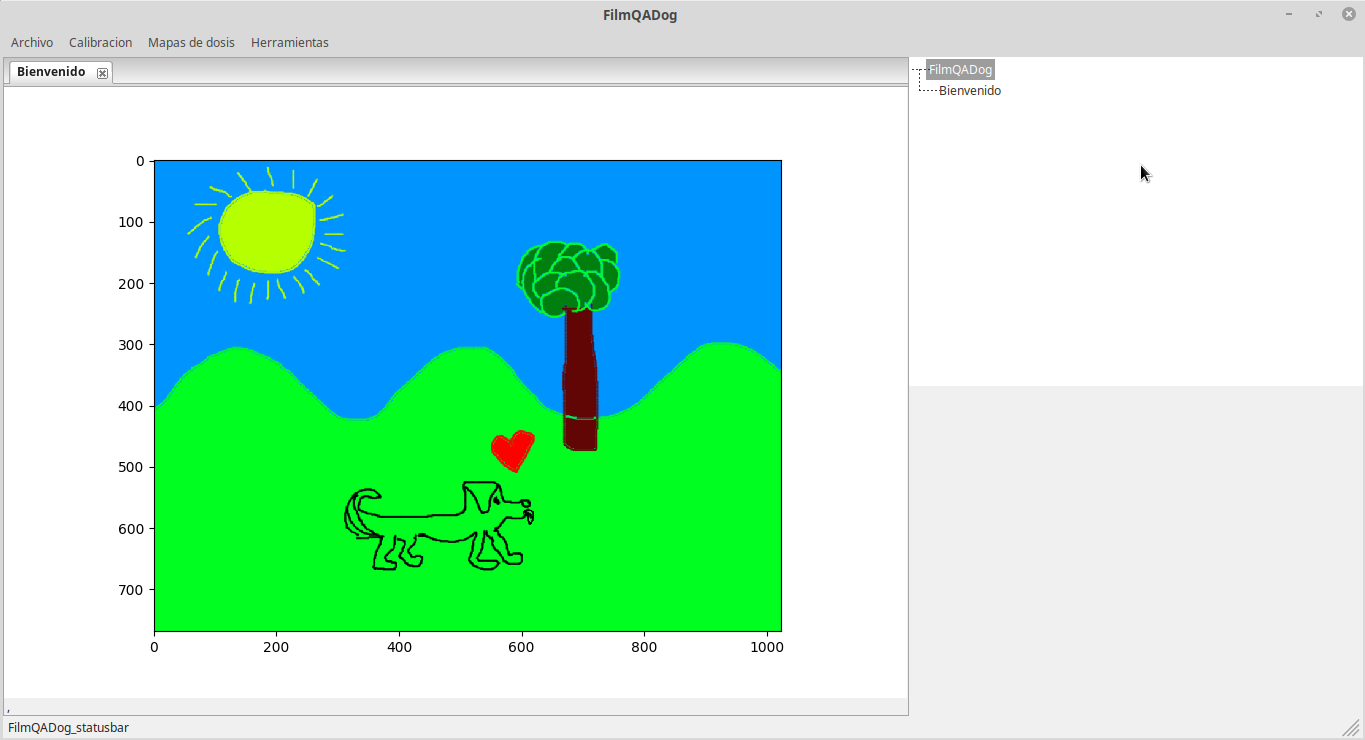
\includegraphics[width=0.7\linewidth]{images/imagenesDocumentacion/ventanaPrincipal.png}
	\caption{Ventana principal }
	\label{fig:ventanaPrincipal}
\end{figure}

En el menú superior se encuentran categorizadas las diversas funcionalidades que se requieren para realizar un análisis con películas radiocrómicas. En la parte derecha se encuentra un árbol de archivos que permite navegar entre los archivos abiertos actualmente en el programa, además del espacio del panel de control, donde se van a ubicar los botones de control dependiendo de la función requerida.\\

El primer menú permite realizar la calibración bajo diferentes configuraciones a partir de una serie de películas irradiadas con diferentes dosis escaneadas en un formato tiff. En la figura \ref{fig:menuCalibracion} se muestran las diferentes opciones de configuración a las cuales el usuario tiene acceso.\\
\begin{figure}[H]
	\centering
	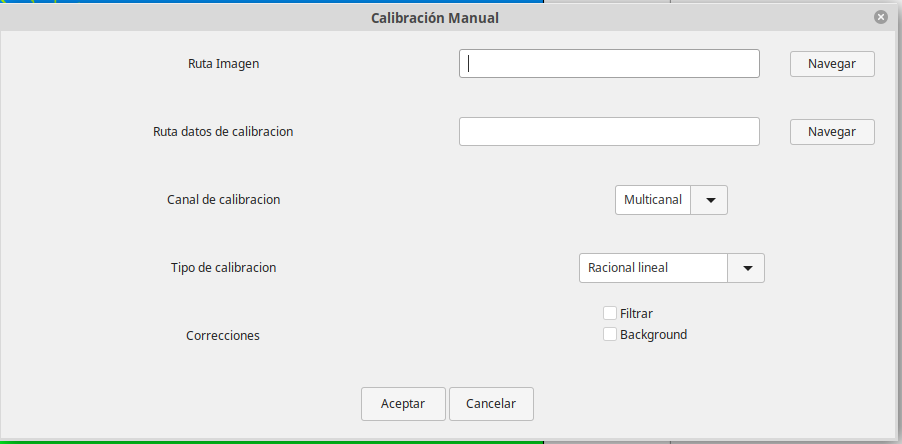
\includegraphics[width=0.7\linewidth]{images/imagenesDocumentacion/menuCalibracion.png}
	\caption{Menú de calibración }
	\label{fig:menuCalibracion}
\end{figure}

Después de la elección de configuración se procede a la ventana de selección de ROI que se usarán en la calibración. Esta ventana se muestra en la imagen \ref{fig:menuEleccionDosis}.
\begin{figure}[H]
	\centering
	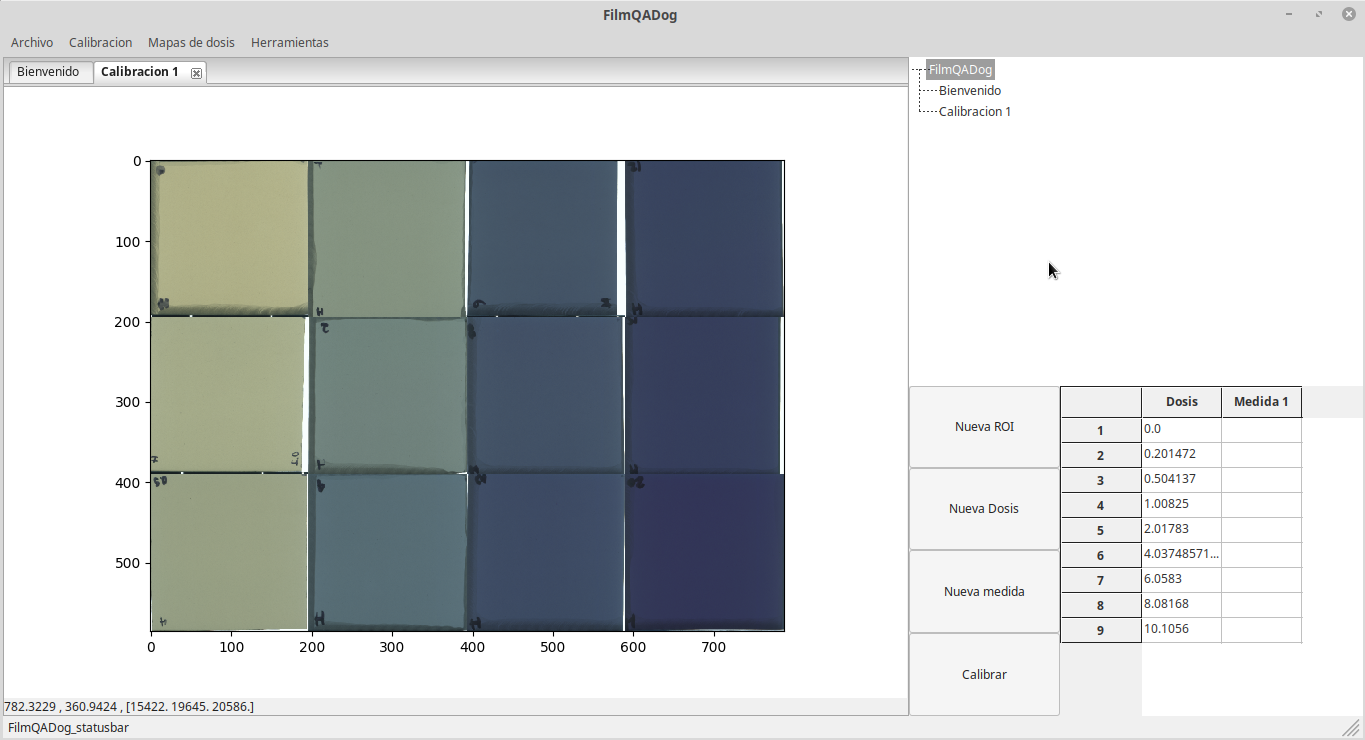
\includegraphics[width=0.7\linewidth]{images/imagenesDocumentacion/menuEleccionDosis.png}
	\caption{Ventana de selección de ROI }
	\label{fig:menuEleccionDosis}
\end{figure}
Pulsando el botón de calibrar se creará un archivo de calibración(con extensión .calibr) que contiene la información del ajuste realizado con los datos que se consignan en la table mediante la interacción con la interfaz. Cada vez que se presione el botón de Nuevo ROI se promediara en la imagen las transmitancias del área elegida y se consignará este valor en la tabla.